\section{\textbf{Results}}
The following simulations were done with an incident plane wave of direction 
$(\theta_i,\phi_i) = (45^{\circ},0^{\circ})$ on VO$_2$ particles supported by a SiO$_2$ substrate
with truncation ratio $t_r = 0$. The surrounding medium is air with $\varepsilon = 1$,
see Figure \ref{fig:simulationFigure}.
The particles are arranged in a square lattice with lattice constant $L = 45$nm and the
particle-particle interaction is given by a dipole contribution. The multipole truncation
is set to $M = 16$.
%
\begin{figure}[h!]
    \centering
    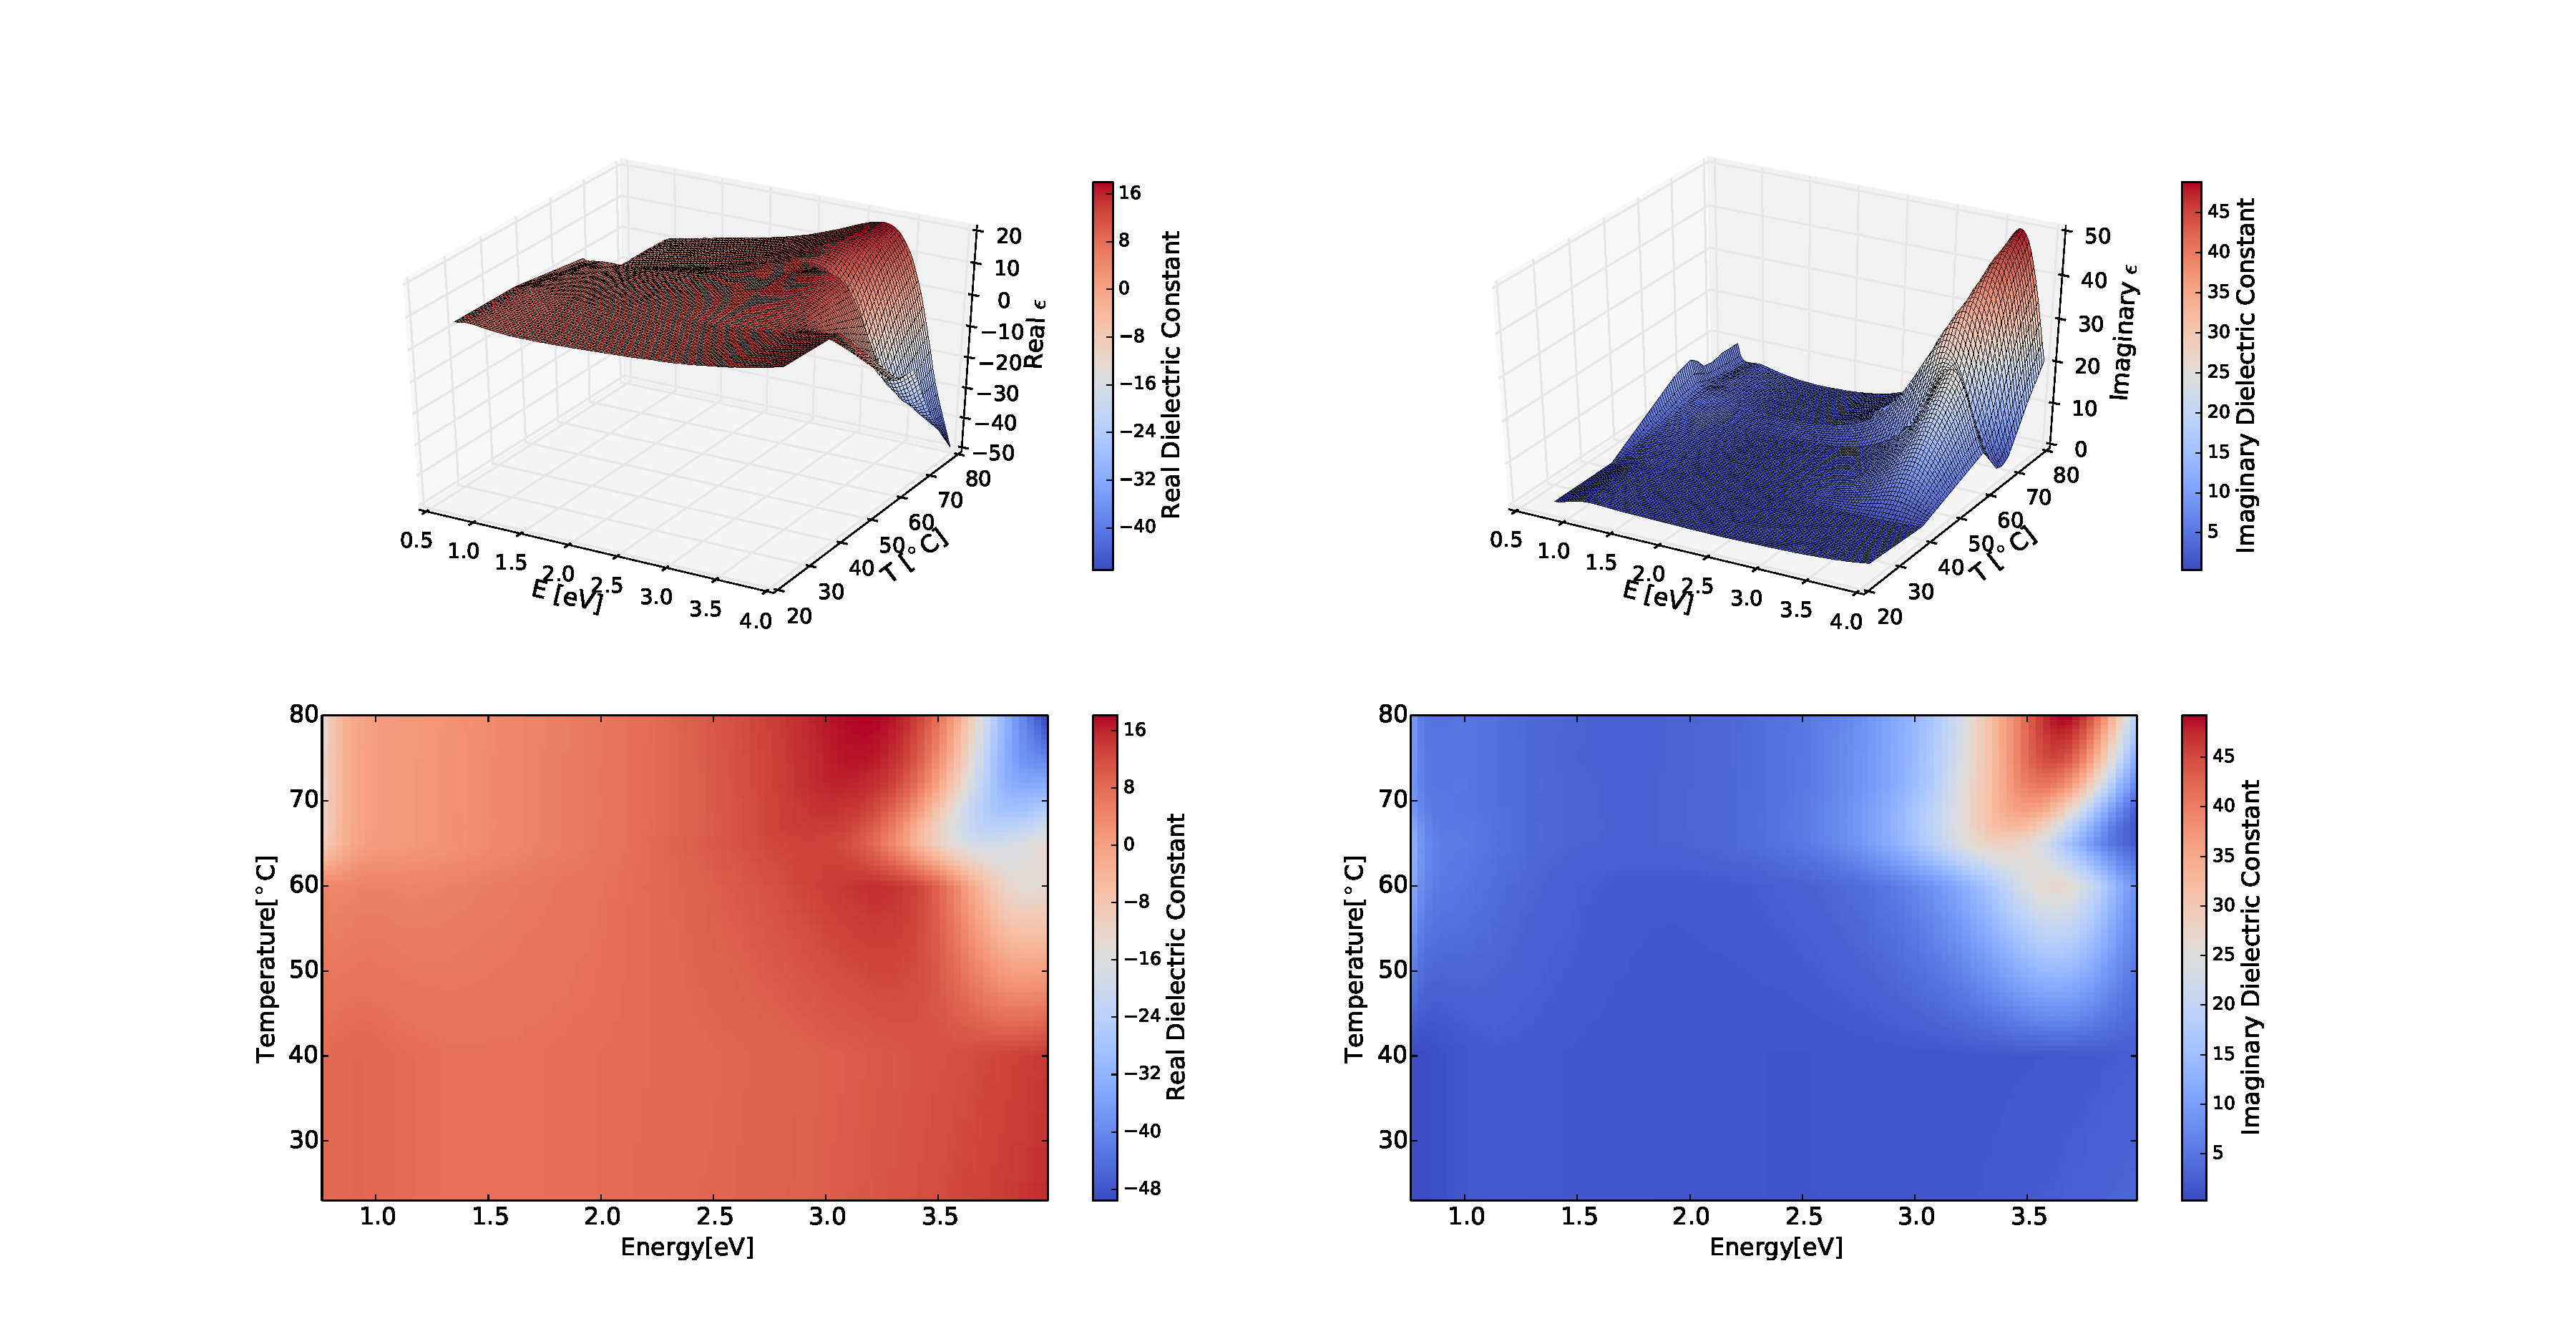
\includegraphics[width=1.1\textwidth]{Results/interpPermittivity.png}
    \caption{
       The interpolated dielectric function $\varepsilon(E,T)$ extracted from 
       Kang et al. \cite[p.~3]{Kang2012}.
    }
    \label{fig:DF}
\end{figure}
%
% Differential reflectance r=10,r=15, s,p
\begin{figure}[h!]
    \centering
    \begin{subfigure}[b]{0.49\textwidth}
        \centering
        \includegraphics[width=\textwidth]{Results/Sim1/dR.pdf}
        \caption{$r = 10$, p-polarization.}
        \label{fig:dR10p}
    \end{subfigure}
    %\hfill
    \begin{subfigure}[b]{0.49\textwidth}
        \centering
        \includegraphics[width=\textwidth]{Results/Sim2/dR.pdf}
        \caption{$r = 10$, s-polarization.}
        \label{fig:dR10s}
    \end{subfigure}
    %\hfill
    \begin{subfigure}[b]{0.49\textwidth}
        \centering
        \includegraphics[width=\textwidth]{Results/Sim3/dR.pdf}
        \caption{$r = 15$, p-polarization.}
        \label{fig:dR15p}
    \end{subfigure}
    %\hfill
    \begin{subfigure}[b]{0.49\textwidth}
        \centering
        \includegraphics[width=\textwidth]{Results/Sim4/dR.pdf}
        \caption{$r = 15$, s-polarization.}
        \label{fig:dR15s}
    \end{subfigure}
    \caption{Relative reflectance $\Delta R/R$ For different radii. The temperatures are chosen in order to
    show the behavior as the temperature increases.}
    \label{fig:dR}
\end{figure}
%
Figure \ref{fig:dR} shows the surface differential reflectivity
\begin{align}
   \frac{\Delta R}{R} = \frac{R-R_0}{R_0}
\end{align}
where $R$ is the total reflectivity and $R_0$ is the bare sufrace, or Fresnel, reflectivity \cite{Lazzari2001}.

%
\begin{figure}[h!]
    \centering
    \begin{subfigure}[b]{0.49\textwidth}
        \centering
        \includegraphics[width=\textwidth]{Results/Sim1/dR_lowE.pdf}
        \caption{$r=10$nm, p-polarization}
        \label{fig:dRlowE1}
    \end{subfigure}
    %\hfill
    \begin{subfigure}[b]{0.49\textwidth}
        \centering
        \includegraphics[width=\textwidth]{Results/Sim2/dR_lowE.pdf}
        \caption{$r=10$nm, s-polarization}
        \label{fig:dRlowE2}
    \end{subfigure}
    %\hfill
    \begin{subfigure}[b]{0.49\textwidth}
        \centering
        \includegraphics[width=\textwidth]{Results/Sim3/dR_lowE.pdf}
        \caption{$r=15$nm, p-polarization}
        \label{fig:dRlowE3}
    \end{subfigure}
    %\hfill
    \begin{subfigure}[b]{0.49\textwidth}
        \centering
        \includegraphics[width=\textwidth]{Results/Sim4/dR_lowE.pdf}
        \caption{$r=15$nm, s-polarization}
        \label{fig:dRlowE4}
    \end{subfigure}
    \caption{Relative reflectance in the IR region $\Delta R/R$.}
    \label{fig:dRlowE}
\end{figure}
%

There are two resonances, one in the IR or low energy region and one at higher energies, just above the
visible region. The peak of the IR resonance is fairly stationary, shifting slightly to the right for 
increasing temperature, before shifting a bit back again. See Figure \ref{fig:dRlowE}. 
Looking back at Figure \ref{fig:dR}, one can see a more dramatic change in the resonance located
above the visible region. The top of the peak is first seen of about 45$^{\circ}$C and shifts to
higher energies with increasing amplitude to about 55-65$^{\circ}$C. For higher temperatures
the response decrease and, based on Figure \ref{fig:dR10p} and \ref{fig:dR10s}, it seems as
the peak of the amplitude shifts back to lower energies.

%
\begin{figure}[h!]
    \centering
    \begin{subfigure}[b]{0.49\textwidth}
        \centering
        \includegraphics[width=\textwidth]{Results/Sim1/dR_IRpeak_amp2.pdf}
        \caption{$r=10$nm, p-polarization}
        \label{fig:IRpeak1}
    \end{subfigure}
    %\hfill
    \begin{subfigure}[b]{0.49\textwidth}
        \centering
        \includegraphics[width=\textwidth]{Results/Sim2/dR_IRpeak_amp2.pdf}
        \caption{$r=10$nm, s-polarization}
        \label{fig:IRpeak2}
    \end{subfigure}
    %\hfill
    \begin{subfigure}[b]{0.49\textwidth}
        \centering
        \includegraphics[width=\textwidth]{Results/Sim3/dR_IRpeak_amp2.pdf}
        \caption{$r=15$nm, p-polarization}
        \label{fig:IRpeak3}
    \end{subfigure}
    %\hfill
    \begin{subfigure}[b]{0.49\textwidth}
        \centering
        \includegraphics[width=\textwidth]{Results/Sim4/dR_IRpeak_amp2.pdf}
        \caption{$r=15$nm, s-polarization}
        \label{fig:IRpeak4}
    \end{subfigure}
    \caption{The IR resonance's peak amplitude of $\Delta R/R$, see Figure \ref{fig:dRlowE}.}
    \label{fig:IRpeak}
\end{figure}
%
%
Based Figure \ref{fig:dR},\ref{fig:dRlowE} and \ref{fig:IRpeak}, one can see that 
the general behavior of the granular thermochromic layer is approximately the same, except for
the amplitude. Because of these similarities, only the 
results for $r = 15$ will be explored further, as the reflective response is larger and therefore more 
interesting.

\newpage
\subsection{Simulation 3; $R = 15$nm, p-polarized incident light}

%
\begin{figure}[h!]
    \centering
    \begin{subfigure}[b]{0.49\textwidth}
        \centering
        \includegraphics[width=\textwidth]{Results/Sim3/re_alpha_parallel.pdf}
        \caption{Re($\alpha_{\parallel})$}
        \label{fig:2}
    \end{subfigure}
    %\hfill
    \begin{subfigure}[b]{0.49\textwidth}
        \centering
        \includegraphics[width=\textwidth]{Results/Sim3/im_alpha_parallel.pdf}
        \caption{Im($\alpha_{\parallel}$)}
        \label{fig:2}
    \end{subfigure}
    %\hfill
    \begin{subfigure}[b]{0.49\textwidth}
        \centering
        \includegraphics[width=\textwidth]{Results/Sim3/re_gamma.pdf}
        \caption{Re($\gamma$)}
        \label{fig:2}
    \end{subfigure}
    %\hfill
    \begin{subfigure}[b]{0.49\textwidth}
        \centering
        \includegraphics[width=\textwidth]{Results/Sim3/im_gamma.pdf}
        \caption{Im($\gamma$)}
        \label{fig:2}
    \end{subfigure}
    \caption{
       The perpendicular polarizability  $\alpha_{\perp}$ and the surface susceptibility $\beta$.
    }
    \label{fig:alphaBeta}
\end{figure}
%
%
\begin{figure}[h!]
    \centering
    \begin{subfigure}[b]{0.49\textwidth}
        \centering
        \includegraphics[width=\textwidth]{Results/Sim3/re_alpha_perp.pdf}
        \caption{Re($\alpha_{\perp}$)}
        \label{fig:}
    \end{subfigure}
    %\hfill
    \begin{subfigure}[b]{0.49\textwidth}
        \centering
        \includegraphics[width=\textwidth]{Results/Sim3/im_alpha_perp.pdf}
        \caption{Im($\alpha_{\perp}$)}
        \label{fig:}
    \end{subfigure}
    %\hfill
    \begin{subfigure}[b]{0.49\textwidth}
        \centering
        \includegraphics[width=\textwidth]{Results/Sim3/re_beta.pdf}
        \caption{Re($\beta$)}
        \label{fig:2}
    \end{subfigure}
    %\hfill
    \begin{subfigure}[b]{0.49\textwidth}
        \centering
        \includegraphics[width=\textwidth]{Results/Sim3/im_beta.pdf}
        \caption{Im($\beta$)}
        \label{fig:2}
    \end{subfigure}
    \caption{
       The parallel polarizability  $\alpha_{\parallel}$ and the surface susceptibility $\gamma$.
    }
    \label{fig:alphaGamma}
\end{figure}
%
The surface polarizability and susceptibility is shown in Figure 
\ref{fig:alphaGamma}, \ref{fig:alphaBeta}. Both the parallel and perpendicular polarizability 
increases substantially for energies lower than 1.0 eV and higher than 2.5 eV. Between 1.0 to 2.0 eV,
however, it experiences a decrease.

%
\begin{figure}[h!]
    \centering
    \begin{subfigure}[b]{0.49\textwidth}
        \centering
        \includegraphics[width=\textwidth]{Results/Sim3/real_gammaDalpha.pdf}
        \caption{re($\alpha_{\perp}$)}
        \label{fig:2}
    \end{subfigure}
    %\hfill
    \begin{subfigure}[b]{0.49\textwidth}
        \centering
        \includegraphics[width=\textwidth]{Results/Sim3/im_gammaDalpha.pdf}
        \caption{im($\alpha_{\perp}$)}
        \label{fig:2}
    \end{subfigure}
    %\hfill
    \begin{subfigure}[b]{0.49\textwidth}
        \centering
        \includegraphics[width=\textwidth]{Results/Sim3/real_betaDalpha.pdf}
        \caption{}
        \label{fig:2}
    \end{subfigure}
    %\hfill
    \begin{subfigure}[b]{0.49\textwidth}
        \centering
        \includegraphics[width=\textwidth]{Results/Sim3/im_betaDalpha.pdf}
        \caption{}
        \label{fig:2}
    \end{subfigure}
    \caption{
       The ratio between the surface polarizabilities and the corresponding surface susceptibilities.
    }
    \label{fig:gammaBetaAlpha}
\end{figure}
%

%
\begin{figure}[h!]
    \centering
    \begin{subfigure}[b]{\textwidth}
        \centering
        \includegraphics[width=\textwidth, trim={2.7cm 0.3cm 4cm 1.3cm},clip]{Results/Sim3/integratedReflectance.pdf}
        \caption{$\theta_i = 45^{\circ}$}
        \label{fig:dR10p}
        \vspace*{1cm}
    \end{subfigure}
    \begin{subfigure}[b]{\textwidth}
        \centering
        \includegraphics[width=\textwidth, trim={2.7cm 0.3cm 4cm 1.3cm},clip]{Results/Sim3/integratedReflectance_theta0.pdf}
        \caption{$\theta = 0_i^{\circ}$}
        \label{fig:dR15s}
    \end{subfigure}
    \caption{
       The integrated reflectance R for both p- and s-polarization. For each subfigure, simulated for
       different angle of incidence, the above figures show the integrated reflectance in the visible
       region 380-780nm, while the lower figures show for 780nm to about 1600nm in the near IR region.
    }
    \label{fig:dR}
\end{figure}
%
%
\begin{figure}[h!]
    \centering
    \begin{subfigure}[b]{\textwidth}
        \centering
        \includegraphics[width=\textwidth, trim={2.5cm 0.3cm 4cm 1.1cm},clip]{Results/Sim3/integratedTransmittance.pdf}
        \caption{$\theta_i = 45^{\circ}$}
        \label{fig:dR10p}
        \vspace*{1cm}
    \end{subfigure}
    \begin{subfigure}[b]{\textwidth}
        \centering
        \includegraphics[width=\textwidth, trim={2.5cm 0.3cm 4cm 1.1cm},clip]{Results/Sim3/integratedTransmittance_theta0.pdf}
        \caption{$\theta = 0_i^{\circ}$}
        \label{fig:dR15s}
    \end{subfigure}
    \caption{
       The integrated transmittance T for both p- and s-polarization. For each subfigure, simulated for
       different angle of incidence, the above figures show the integrated reflectance in the visible
       region 380-780nm, while the lower figures show for 780nm to about 1600nm in the near IR region.
    }
    \label{fig:dR}
\end{figure}
%

\begin{thebibliography}{9}

   \bibitem{Lazzari2001}
   Lazzari R, Simonsen I, Bedeaux D, Vlieger J, Jupille J.
   Polarizability of truncated spheroidal particles supported by a substrate: model and applications.
   The European Physical Journal B 2001; 24:267-284
\end{thebibliography}



